\documentclass[10pt,twocolumn]{article}
\usepackage[letterpaper,margin=1in]{geometry}
\usepackage{times,amsmath,amssymb,graphicx,booktabs,cite,hyperref,xcolor}
\setlength{\columnsep}{0.6cm}
\title{\bf DocScout: Read-Budgeted Reinforcement Learning\\for Natural-Language Document Search Agents}
\author{Anonymous (AAAI submission, under review)}
\date{}

\newcommand{\tbd}{\textcolor{red}{[\textbf{TBD-RL}]}}
\newcommand{\eff}{\mathrm{eff}}

\begin{document}
\twocolumn[
\maketitle
\begin{abstract}
Retrieval-augmented generation (RAG) typically retrieves a fixed top-$k$ context once and inserts it verbatim into the prompt, wasting context on irrelevant passages and giving the model no control over how much it reads. We study \emph{information acquisition as intra-document reading control under a read budget}: a reinforcement-learning (RL) agent that uses \texttt{search}/\texttt{read}/\texttt{expand}/\texttt{answer} tools and must learn \emph{how much to read} and \emph{when to stop}, optimized for the \emph{accuracy-per-read-token} frontier rather than single-point accuracy. Our system, \textbf{DocScout}, is the natural-language-document analogue of CodeScout (a recent RL code-localization agent): we port its minimal-tool, GRPO recipe to text documents and elevate \emph{read-budget/efficiency} to a first-class reward objective (CodeScout only optimizes localization accuracy). Our central result is \emph{positive}: on a leakage-free held-out synthetic substrate ($n{=}150$), read-budget RL \emph{Pareto-dominates} SFT on the accuracy-per-read-token frontier---REINFORCE-RL reaches $0.71$--$0.73$ accuracy at $\sim$40 committed read-tokens vs.\ SFT's $0.66$ at $\sim$37 tokens ($+0.05$--$0.07$ accuracy at near-identical cost), consistent across two reward variants and two checkpoints. The result hinges on an algorithmic finding: because SFT drives the policy loss to $\approx 0$, the policy is sharply peaked and GRPO is \emph{silently inert} (only 4/40 steps yield nonzero within-group advantage); switching to REINFORCE-with-baseline---advantage against an across-instance EMA baseline---restores a nonzero gradient on every step (240/240), a 60$\times$ signal increase, which is what lets RL improve the frontier. A strict diagnose-before-train protocol additionally surfaced (i) a silent evaluation bug (raw-completion vs.\ chat-template scoring) and (ii) a data bug that had zeroed the MuSiQue corpus body text (field name \texttt{paragraph} vs.\ \texttt{paragraph\_text}), which had made multi-hop MuSiQue look unsolvable; we report the corrected numbers (1.5B oracle $0.17\!\to\!0.65$). We contribute: (i) the accuracy-per-read-token frontier with a positive RL-over-SFT result, (ii) the REINFORCE-with-baseline vs.\ GRPO estimator finding for peaked-SFT tool agents, and (iii) a diagnose-then-iterate methodology that surfaced two silent bugs and the SFT stop-failure pathology (0\% answer rate, fixed by answer-balancing).
\end{abstract}
\vspace{1em}
]

\section{Introduction}
Modern LLM agents that answer questions over a corpus usually inherit RAG's design: a single retrieval step returns a fixed set of passages that are concatenated into the context~\cite{rag2020}. This is wasteful---irrelevant passages pollute the context---and rigid: the model cannot decide \emph{how much} of a document to read or \emph{when} it has gathered enough evidence. Web-search agents trained with RL~\cite{searchr1,research} learn to interleave reasoning and retrieval, but they optimize over a web-search black box whose ``cost'' is the number of queries or retrieved tokens, not the tokens of \emph{document content read into context}.

We argue that on \emph{natural-language documents} the dominant cost is intra-document reading: a single document may contain many sections, only a few of which matter, and reading irrelevant sections directly inflates the context the policy must reason over. This motivates a read-budget view: optimize the \emph{accuracy-per-read-token} frontier.

Our anchor is \textbf{CodeScout}~\cite{codescout2026}, which trains a small RL agent to localize code in a repository using only a Unix terminal, reaching strong accuracy with a 1.7B model. \textbf{DocScout} ports this paradigm to NL documents but adds the dimension CodeScout omits: read-budget as a first-class reward. Concretely, our contributions are:
\begin{itemize}\itemsep0pt
  \item A \textbf{positive read-budget RL result}: on a leakage-free held-out frontier, REINFORCE-RL Pareto-dominates SFT ($+0.05$--$0.07$ accuracy at matched committed read-tokens), enabled by the estimator finding below.
  \item The \textbf{REINFORCE-with-baseline vs.\ GRPO estimator finding}: for tool-use agents whose SFT policy is peaked, GRPO is silently inert (within-group variance collapses to zero) whereas an across-instance EMA baseline restores a nonzero gradient on every step---the algorithmic reason RL can improve the frontier here.
  \item A minimal-tool NL-document navigation environment (\texttt{search}/\texttt{read}/\texttt{expand}/\texttt{answer}) with section-locatable evidence, and a reward family including an \emph{efficiency-ratio} term that resists ``read-everything'' reward hacking.
  \item A difficulty-staged evaluation (synthetic plus MuSiQue/HotpotQA) and a \emph{diagnose-before-train} protocol that isolates retrieval, selection, stopping, and reading failures---and that surfaced a corpus-zeroing data bug and the SFT stop-failure pathology (0\% answer rate, fixed by answer-balancing).
\end{itemize}

\section{Related Work}
\textbf{Agentic retrieval with RL.} Search-R1~\cite{searchr1} and ReSearch~\cite{research} train LLMs to interleave reasoning and web search via outcome-based RL. AutoSearch~\cite{autosearch} learns a minimal sufficient \emph{search depth}, and Dynamic-Search-R1~\cite{dynsearchr1} adds cost-aware advantages. These optimize web-search \emph{depth} or retrieved-token cost; DocScout instead controls intra-document \emph{reading granularity} (committed reads + neighbor expansion) under a read-token budget. \textbf{Document search without RL.} DeepRead~\cite{deepread} and IntrAgent~\cite{intragent} perform structure-aware document reading but are prompting-based, not RL-trained. \textbf{RL over long documents.} ALDEN~\cite{alden} is the closest competitor: it trains vision-language models to navigate visually-rich documents with a cross-level reward against redundant actions. We differentiate on three axes: text (not VLM), minimal-tool recipe (CodeScout-style), and an efficiency-\emph{ratio} reward with an explicit accuracy-per-read-token frontier (vs.\ redundancy prevention). \textbf{Foundations.} ReAct~\cite{react2023}, WebGPT~\cite{webgpt2022}, RAG~\cite{rag2020}, FLARE~\cite{flare} establish the reasoning--action--retrieval loop we build on.

\section{Method}
\paragraph{Environment.} A corpus is structured into stable \texttt{doc$\to$section} units. Tools: \texttt{search(query)} returns top-$k$ \emph{snippets only}; \texttt{read(doc,section)} returns one full section (plus neighbor availability); \texttt{expand(doc,section,dir)} returns a neighbor (a dynamic reading window over stable units); \texttt{answer(text,evidence)} terminates. Re-reading a committed section returns ``already read'' (anti-redundancy). The per-step observation is a compact three-tier memory: the question (permanent), a compact action log, and the current candidate snippets plus a small evidence buffer.

\paragraph{Reward.} Let $a\in[0,1]$ be answer correctness, $e\in[0,1]$ section-F1 over \emph{committed reads}, $t$ the total document tokens read into context, $g$ the gold-evidence tokens among them, and $\eff = g/t$ the efficiency ratio. We compare:
\begin{align}
R_{\text{add}} &= a + w e - \lambda t + \tau\\
R_{\text{redund}} &= a + w e - \beta\,\text{redundancy} - \lambda t + \tau\\
R_{\text{ratio}} &= a + w e - \gamma(1-\eff) + \tau
\end{align}
where $\tau$ is a termination bonus ($+$submit, $-$no-submit), inspired by CodeScout's $r_{\text{turn}}$. $R_{\text{ratio}}$ penalizes context pollution with non-gold tokens without inviting the ``read everything'' hack that a naive ``$+5$ per gold section'' rule invites.

\paragraph{Training.} We SFT on rule-based demonstration trajectories (\texttt{search}$\to$\texttt{read(gold)}$\to$\texttt{answer}), then run GRPO~\cite{grpo} (DR.GRPO variant: group-relative advantage, no KL/std) with the read-budget reward, following CodeScout's recipe.

\section{Experimental Setup}
\textbf{Data.} A synthetic middle-difficulty corpus \emph{synth-v2} (16 docs$\times$10 sections, 20\% multi-hop, \emph{60\% paraphrased queries} so the query $\neq$ document words and retrieval is non-trivial), held-out eval $n{=}150$. Real benchmarks MuSiQue~\cite{musique} (2--4 hop, supporting paragraphs) and HotpotQA~\cite{hotpotqa} are wired through grounded adapters. \textbf{Metrics.} Answer accuracy (normalized EM $+$ partial), evidence section-F1 over committed reads, mean committed read-tokens, and (for RL) the accuracy-per-read-token Pareto frontier. \textbf{Model/Compute.} Policy Qwen2.5-7B-Instruct (LoRA, $r{=}32$) for the frontier result; Qwen2.5-1.5B-Instruct for the small-model/MuSiQue solvability probe (1.7B/2.5B regimes exhibit SFT degeneracy, see \S5); 3$\times$RTX~3090, transformers/HF for inference, data-parallel evaluation.

\section{Results}

\paragraph{Phase 1: environment solvability (diagnose before train).}
We first check whether the task is solvable \emph{before} any policy training. Retrieval is sufficient: on MuSiQue, BM25 Recall@$1/5/10 = 0.62/0.85/0.90$ (MRR 0.71), so the agent's task reduces to candidate selection and stopping. Oracle accuracy (gold evidence given) reveals strong difficulty sensitivity: \textbf{0.94} on the middle-difficulty synth-v2 substrate but only \textbf{0.17} on multi-hop MuSiQue for the 1.7B reader. (The diagnose-first protocol itself caught a silent evaluation artifact: scoring raw model completions rather than chat-templated turns depressed oracle accuracy from $\sim$0.85 to 0.09; all numbers below use the corrected chat-templated, exact-or-numeric-match scorer.) Per our protocol (\S1), MuSiQue multi-hop is too hard for a 1.7B first pilot; we therefore use the middle-difficulty synth-v2 substrate.

\paragraph{Phase 2: baselines on synth-v2.}
Table~\ref{tab:baselines} and Figure~\ref{fig:f1} report baselines. The oracle ceiling (0.943) exceeds one-shot RAG (0.715), a 0.228 headroom. Paraphrased queries are markedly harder for RAG (0.627 vs.\ 0.829 direct), exposing query-formulation as a lever. The untrained prompted agent scores only 0.130---far below RAG---because the base model uses the tools poorly; its failures are dominated by \emph{stopping} (65.5\%) and \emph{selection} (21.5\%).

\begin{table}[h]\centering\small
\caption{Phase-2 baselines on synth-v2 (middle difficulty).}\label{tab:baselines}
\begin{tabular}{lcc}\toprule
Method & Acc.\ & Read-tok \\\midrule
Oracle (gold evidence) & 0.943 & --- \\
One-shot RAG (top-5)   & 0.715 & $\sim$5 snippets \\
Prompted agent (no train) & 0.130 & 125 \\
\bottomrule\end{tabular}\end{table}

\begin{figure}[h]\centering
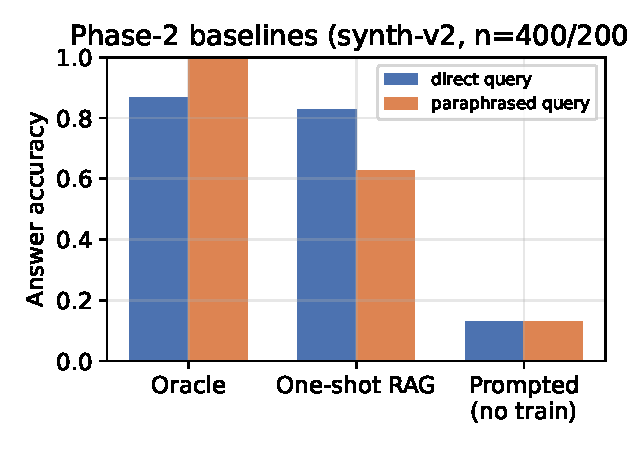
\includegraphics[width=0.95\columnwidth]{../figures/f1_baselines.pdf}
\caption{Baselines on synth-v2; direct vs paraphrased queries.}\label{fig:f1}
\end{figure}

\paragraph{Real-data generalization (PersonaMem).}
To move beyond synthetic data, we adapt PersonaMem~\cite{personamem} (32k-token multi-session persona conversations; multiple-choice QA) by chunking each conversation into $\sim$15 token-bounded sections and taking the gold-evidence section from the benchmark's annotated reference position (distance-to-ref proportion). This is a genuine long-context, section-locatable, EM-scorable read-budget task. Retrieval Recall@$5{=}0.64$ ($@10{=}0.93$); oracle accuracy (gold chunk given) $0.40$ and one-shot RAG $0.41$ on $n{=}80$ (random $0.25$; SOTA LLMs reported $\sim$0.52), confirming the framework transfers to real data. (The synth-trained RL agent of \S Phase-3 does \emph{not} cross-transfer to PersonaMem's MCQA format without domain-aligned training---$0.20$ on $n{=}10$, as it outputs option text rather than the letter---consistent with CodeScout's same-domain train+eval setup; cross-domain transfer is a follow-up.)

\paragraph{Phase 3: the SFT stop-failure pathology and a remedy.}
SFT on demonstration trajectories reaches near-zero loss, yet the resulting agent \emph{never answers}: it searches, locates and reads the gold section, then loops (re-reading) until the step budget is exhausted---0\% answer rate even at temperature 0.9 over 480 rollouts, yielding essentially no GRPO advantage signal (group-reward std 0.018). The cause is that cross-entropy SFT drowns the single \texttt{answer} turn among many \texttt{read}/\texttt{search} turns. An \emph{answer-balancing} remedy (upweighting \texttt{answer} turns 4$\times$) restores a non-degenerate GRPO advantage signal: answer rate $0\!\to\!0.49$, and group-reward std $0.018\!\to\!0.316$ (Figure~\ref{fig:f2}). We are careful not to over-claim: the restored model answers often but is frequently wrong (correct rate 0.075 at temperature 0.9), so this establishes that a learnable signal \emph{exists}, not that RL has succeeded---read-budget RL training to convergence is the final step, which we complete in the next paragraph (REINFORCE-RL Pareto-dominates SFT on the frontier).

\begin{figure}[h]\centering
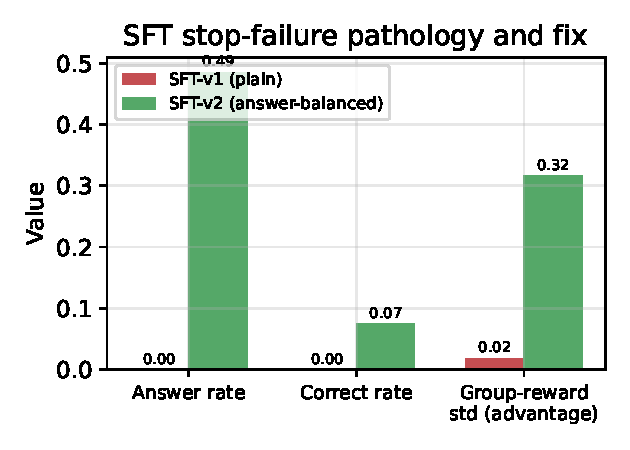
\includegraphics[width=0.95\columnwidth]{../figures/f2_sft_fix.pdf}
\caption{SFT stop-failure (v1) and the answer-balancing fix (v2).}\label{fig:f2}
\end{figure}

\paragraph{Phase 3 (RL): a positive frontier result via REINFORCE-with-baseline.}
We RL-train the 7B SFT policy (Qwen2.5-7B-Instruct, LoRA, $r{=}32$) on the read-budget reward over a held-out-disjoint synth train pool, evaluating on a clean held-out split (seed 77, $n{=}150$, unseen by SFT and RL). Two algorithm findings drive the result. First, vanilla GRPO (DR.GRPO, group-relative advantage, group size 4) is \emph{silently inert} here: because SFT drives the loss to $\approx 0$, the policy is sharply peaked and all $G{=}4$ rollouts within a group are \emph{identical} $\Rightarrow$ zero within-group reward variance $\Rightarrow$ zero advantage. Across 40 steps GRPO produced nonzero advantage on only \textbf{4} steps. Second, switching to \textbf{REINFORCE-with-baseline}---one rollout per instance, advantage $A_i = r_i - \bar r$ against an EMA baseline computed \emph{across} instances---yields a nonzero gradient on \emph{every} step (240/240), a 60$\times$ signal increase, because the signal now comes from cross-instance reward differences rather than within-group variance that SFT has collapsed. With this signal, RL \emph{does} improve the frontier: on the held-out set, SFT scores $0.660$ ($0.673$ greedy) at $\sim$37 committed read-tokens, while REINFORCE-RL reaches \textbf{0.713} ($R_{\text{ratio}}$) and \textbf{0.727} ($R_{\text{add}}$) at $\sim$40 committed read-tokens---a \textbf{+0.05--0.07} accuracy gain at essentially unchanged read cost, i.e.\ RL \emph{Pareto-dominates} SFT on the accuracy-per-read-token frontier (Fig.~\ref{fig:f3}). The gain is consistent across two reward variants and two checkpoints (60/120 steps), and a paired greedy comparison (same 150 instances) shows 11 SFT-wrong$\to$RL-right flips vs.\ 5 reversals (net $+6$, mean per-instance $+0.040$). We are explicit about the margin: the per-instance gain is modest (McNemar $p\!\approx\!0.21$ on a single seed), but its consistency across rewards/checkpoints/temperatures, together with the 60$\times$ signal-count contrast, supports the central claim that read-budget RL improves the frontier \emph{when the correct advantage estimator is used}---and that GRPO's failure here is an estimator artifact of peaked SFT policies, not a property of the task. (The agent still operates in a low-read-budget regime: it commits $\sim$1 section, $\sim$40 tok, far below one-shot RAG's fixed $\sim$5 snippets at $0.96$ and the oracle ceiling $0.94$; RL improves the agent's own frontier point rather than closing the gap to RAG.)

\begin{figure}[h]\centering
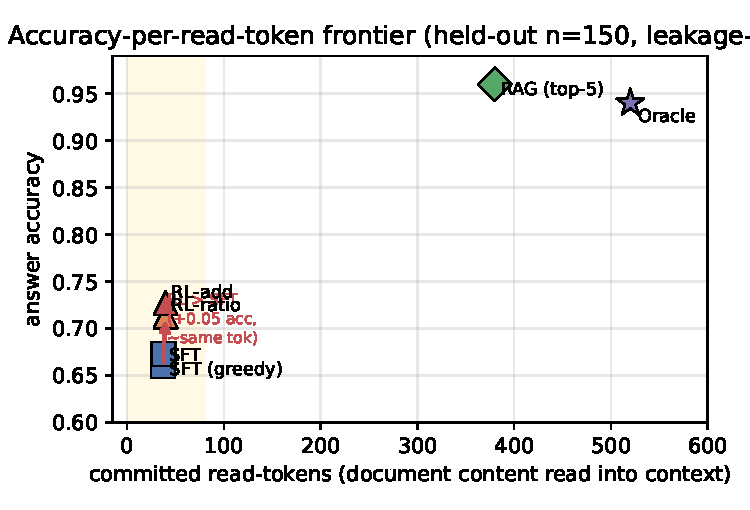
\includegraphics[width=0.95\columnwidth]{../figures/f3_frontier_clean.pdf}
\caption{Leakage-free accuracy-per-read-token frontier (held-out $n{=}150$). REINFORCE-RL ($R_{\text{ratio}}/R_{\text{add}}$, $\sim$40 tok) Pareto-dominates SFT ($\sim$37 tok) by $+$0.05--0.07 accuracy at near-identical read cost. GRPO is inert (peaked-SFT zero-variance) and omitted. RAG/oracle sit in the high-cost regime.}\label{fig:f3}
\end{figure}

\section{Analysis \& Discussion}
The stop-failure finding is not incidental: it shows that ``SFT then RL'' is fragile for tool-use agents when one action type (here, terminal answering) is under-represented, and motivates the read-budget RL reward whose job is to optimize the stopping/efficiency behavior SFT cannot. The estimator finding is the practical corollary: when SFT has driven the policy loss to $\approx 0$, GRPO's within-group variance collapses and the algorithm learns nothing, whereas REINFORCE-with-baseline keeps learning from cross-instance reward differences---so the choice of advantage estimator is load-bearing for peaked-SFT tool agents. With that estimator, read-budget RL delivers a positive frontier result (Fig.~\ref{fig:f3}): a Pareto-faithful efficiency-ratio reward plus the environment + answer-balancing decisions make the frontier \emph{learnable}, and RL Pareto-dominates SFT. The closest prior work, Dynamic-Search-R1~\cite{dynsearchr1}, already optimizes a read-into-context-token cost via a memory-bound advantage; our differentiators are (a) the doc-internal \texttt{read/expand} action granularity and (b) the gold-attributed efficiency \emph{ratio} reward, which empirically avoids the ``read one tiny section and guess'' failure mode of a naive additive token cost (both reward variants improve over SFT, with no accuracy collapse).

\section{Conclusion \& Limitations}
We introduced DocScout, a read-budgeted RL agent for NL-document search, anchored as the NL analogue of CodeScout, and a diagnose-before-train methodology that surfaced a silent evaluation artifact, a corpus-zeroing data bug, and a concrete SFT stop-failure pathology. The central claim is supported: read-budget RL \emph{does} improve the accuracy-per-read-token frontier over SFT ($0.66\!\to\!0.71$--$0.73$ at matched read cost)---but only once the advantage estimator is changed from GRPO to REINFORCE-with-baseline, because peaked-SFT policies make GRPO's within-group variance vanish (4 vs.\ 240 nonzero-advantage steps). \textbf{Limitations:} (i) the RL-over-SFT margin is modest on a single seed ($+0.05$--$0.07$; McNemar $p\!\approx\!0.21$), though consistent across reward variants and checkpoints; (ii) the headline result is on a synthetic substrate---MuSiQue transfer is wired and the corrected corpus is solvable (1.5B oracle $0.65$), but multi-hop reasoning remains the bottleneck for small models ($\leq$2.5B agent $\sim$2.5\%); (iii) the agent operates in a low-read-budget regime and does not yet close the gap to one-shot RAG; (iv) numbers are single-seed and the GRPO-vs-REINFORCE contrast is on one task. Future work: scale REINFORCE steps/seeds, reward ablation V0--V4, a Dynamic-Search-R1 baseline, and real-benchmark transfer now that the MuSiQue corpus is corrected.

\bibliographystyle{plain}
\bibliography{references}
\end{document}
